\section{Suddivisione del lavoro}
I componenti del gruppo dovranno rivestire ciascuno, almeno una volta, tutti i ruoli specificati nell'\textit{organigramma\ped{G}}.
Durante le varie fasi ogni componente può ricoprire più ruoli, anche contemporaneamente, purchè non si presentino dei conflitti di interesse tra le attività svolte. Ad esempio un componente non può essere \textit{\Ver} di se stesso.
\subsection{Analisi dei Requisiti}
Nell'attività di \textit{\AdR} ciascun componente dovrà rivestire i seguenti ruoli:
\begin{table}[H]
	\begin{center}
		\begin{tabular}{|c|c|c|c|c|c|c|c|}
			\hline
			\textbf{Nominativo} & \multicolumn{6}{c|}{\textbf{Ore per ruolo}} & \textbf{Ore totali} \\
			& \textbf{Re} & \textbf{Am} & \textbf{An} & \textbf{Pj} & \textbf{Pr} & \textbf{Ve} & \\
			\hline
			\FB	&		&	4	&	23	&		&		&		&	27	\\
			\hline
			\AF		&		&	6	&	21	&	 	&		&		& 	27	\\
			\hline
			\GN		&	20	&		&	9	&		&		&		&	29	\\
			\hline
			\GR	&	20	&	 	&	8 	&		&	 	& 		&	28	\\
			\hline
			\SM 		&		&	3	&	5	&		&		& 	20	&	28	\\
			\hline
			\MP		& 		&		&	7	&		&		&	20	&	27	\\
			\hline
			\MV 		&		&	4	&	5	&		&		&	20	& 	29	\\
			\hline
		\end{tabular}
	\end{center}
	\caption{Ore per componente, \AdR}
\end{table}

\begin{figure}[H]
	\centering
	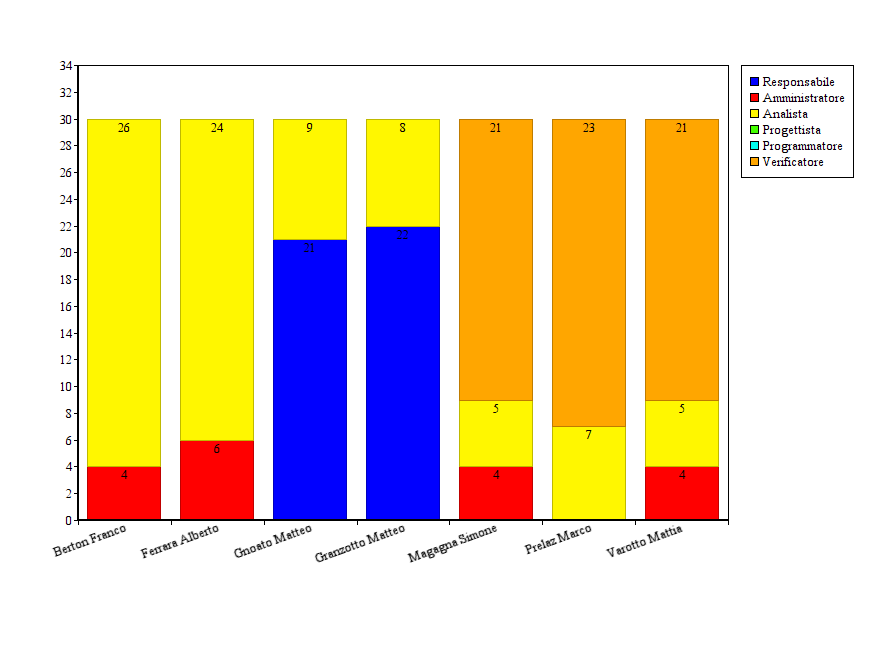
\includegraphics[scale=0.4]{immagini/Grafi/GrafoAR}
	\caption{Incidenza ore per ruolo, Analisi dei Requisiti}
\end{figure}

\subsection{Analisi dei Requisiti in Dettaglio}
Nell'attività di Analisi dei Requisiti in Dettaglio ciascun componente dovrà rivestire i seguenti ruoli:

\begin{table}[H]
	\begin{center}
		\begin{tabular}{|c|c|c|c|c|c|c|c|}
			\hline
			\textbf{Nominativo} & \multicolumn{6}{c|}{\textbf{Ore per ruolo}} & \textbf{Ore totali} \\
			& \textbf{Re} & \textbf{Am} & \textbf{An} & \textbf{Pj} & \textbf{Pr} & \textbf{Ve} & \\
			\hline
			\FB	&		&		&	3	&		&		&		&	3	\\
			\hline
			\AF		&		&		&	3	&	 	&		&		& 	3	\\
			\hline
			\GN		&	1	&		&		&		&		&		&	1	\\
			\hline
			\GR	&	2	&	 	&	 	&		&	 	& 		&	2	\\
			\hline
			\SM 		&		&	1	&		&		&		& 	1	&	2	\\
			\hline
			\MP		& 		&		&		&		&		&	3	&	3	\\
			\hline
			\MV 		&		&		&		&		&		&	1	& 	1	\\
			\hline
		\end{tabular}
	\end{center}
	\caption{Ore per componente, \AD}
\end{table}

\begin{figure}[H]
	\centering
	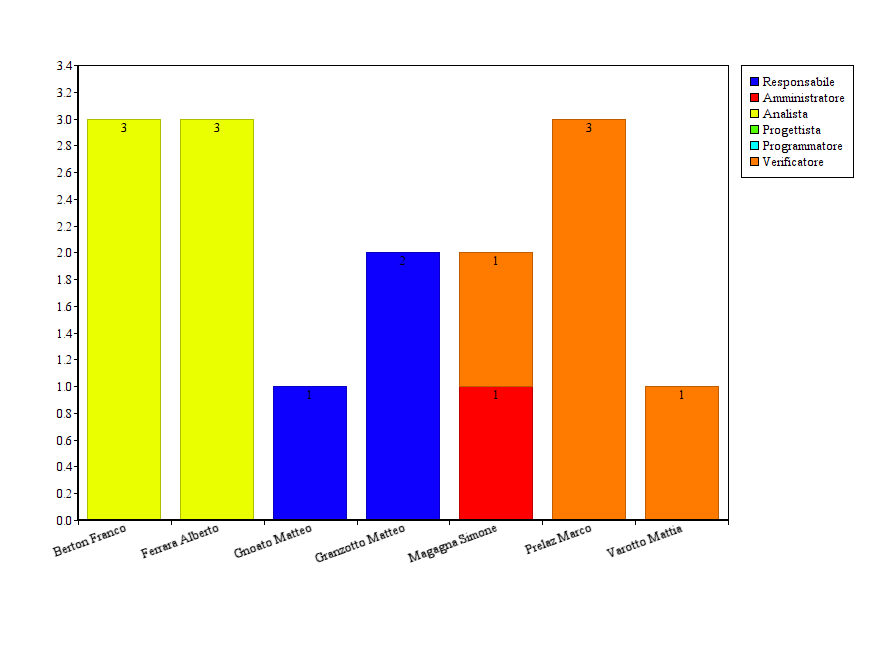
\includegraphics[scale=0.4]{immagini/Grafi/GrafoARD}
	\caption{Incidenza ore per ruolo, \AD}
\end{figure}

\subsection{Progettazione Architetturale}
Nel periodo di Progettazione Architetturale ciascun componente del gruppo dovrà rivestire i seguenti ruoli:
\begin{table}[H]
	\begin{center}
		\begin{tabular}{|c|c|c|c|c|c|c|c|}
			\hline
			\textbf{Nominativo} & \multicolumn{6}{c|}{\textbf{Ore per ruolo}} & \textbf{Ore totali} \\
			& \textbf{Re} & \textbf{Am} & \textbf{An} & \textbf{Pj} & \textbf{Pr} & \textbf{Ve} & \\
			\hline
			\FB		&		&		&		&	10	&		&	23	&	33	\\
			\hline
			\AF	&		&		&		&	9 	&		&	23	& 	32	\\
			\hline
			\GN		&		&		&		&	8	&		&	24	&	32	\\
			\hline
			\GR	&		&	 4	&  		&	28	&	 	& 		&	32	\\
			\hline
			\SM 		&	3	&		&		&	29	&		& 		&	32	\\
			\hline
			\MP 		& 		&	4	&		&	28	&		&		&	32	\\
			\hline
			\MV 		&	3	&		&		&	29	&		&		& 	32	\\
			\hline
		\end{tabular}
	\end{center}
	\caption{Ore per componente, Progettazione Architetturale}
\end{table}

\begin{figure}[H]
	\centering
	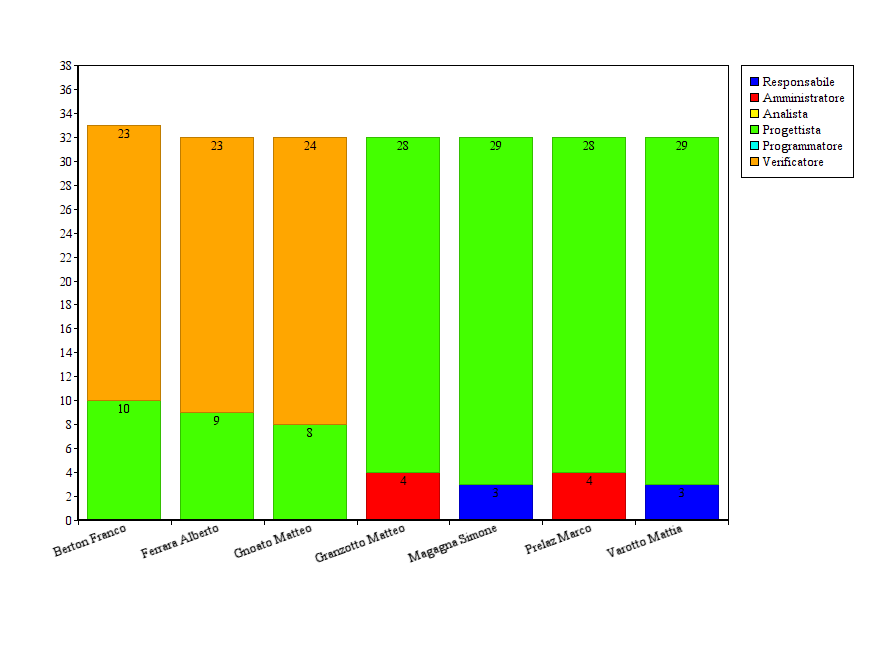
\includegraphics[scale=0.4]{immagini/Grafi/GrafoPA}
	\caption{Incidenza ore per ruolo, Progettazione Architetturale}
\end{figure}

\subsection{Progettazione di Dettaglio}
Nel periodo di Progettazione di Dettaglio ciascun componente del gruppo dovrà rivestire i seguenti ruoli:
\begin{table}[H]
	\begin{center}
		\begin{tabular}{|c|c|c|c|c|c|c|c|}
			\hline
			\textbf{Nominativo} & \multicolumn{6}{c|}{\textbf{Ore per ruolo}} & \textbf{Ore totali} \\
			& \textbf{Re} & \textbf{Am} & \textbf{An} & \textbf{Pj} & \textbf{Pr} & \textbf{Ve} & \\
			\hline
			\FB		&	3	&		&		&	17	&		&		&	20	\\
			\hline
			\AF		&	4	&		&		&	16	&		&		& 	20	\\
			\hline
			\GN		&		&	2	&		&	18	&		&		&	20	\\
			\hline
			\GR	&		&	 	&		&	6	&	 	& 	14	&	20	\\
			\hline
			\SM 		&		&	3	&		&	17	&		& 		&	20	\\
			\hline
			\MP 		& 		&		&		&	6	&		&	14	&	20	\\
			\hline
			\MV 		&		&		&		&	6	&		&	14	& 	20	\\
			\hline
		\end{tabular}
	\end{center}
	\caption{Ore per componente,Progettazione di Dettaglio}
\end{table}

\begin{figure}[H]
	\centering
	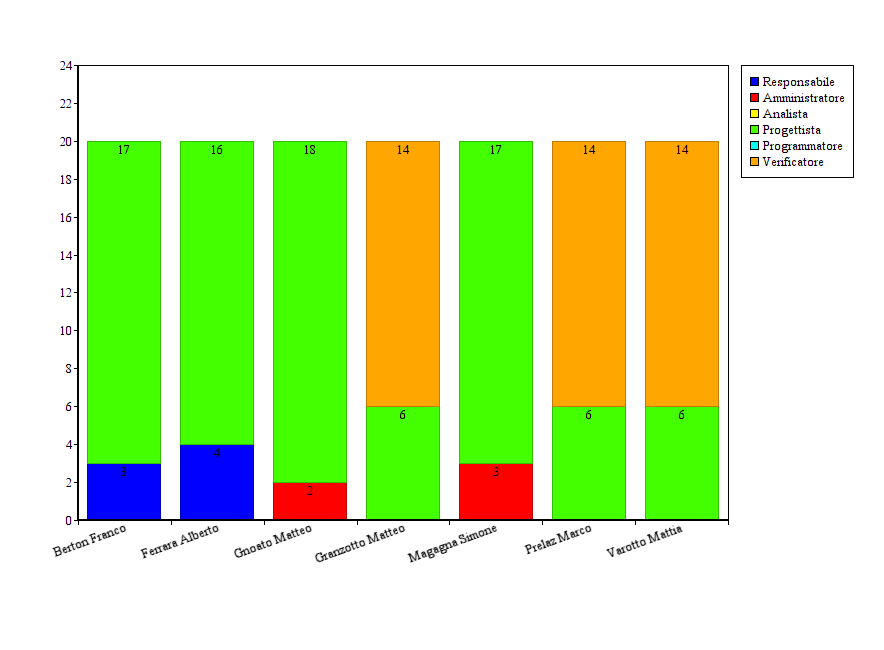
\includegraphics[scale=0.4]{immagini/Grafi/GrafoPD}
	\caption{Incidenza ore per ruolo, Progettazione di Dettaglio}
\end{figure}

\subsection{Codifica}
Nel periodo di Codifica ciascun componente del gruppo dovrà rivestire i seguenti ruoli:
\begin{table}[H]
	\begin{center}
		\begin{tabular}{|c|c|c|c|c|c|c|c|}
			\hline
			\textbf{Nominativo} & \multicolumn{6}{c|}{\textbf{Ore per ruolo}} & \textbf{Ore totali} \\
			& \textbf{Re} & \textbf{Am} & \textbf{An} & \textbf{Pj} & \textbf{Pr} & \textbf{Ve} & \\
			\hline
			\FB		&		&		&		&		&	35	&		&	35	\\
			\hline
			\AF		&		&		&		&	 5	&	31	&		& 	36	\\
			\hline
			\GN		&		&	4	&		&		&	7	&	25	&	36	\\
			\hline
			\GR	&	5	&	 	&		&	5	&	25 	& 		&	35	\\
			\hline
			\SM 		&		&		&		&	5	&	5	& 	25	&	35	\\
			\hline
			\MP 		& 	6	&		&		&	5	&	24	&		&	35	\\
			\hline
			\MV 		&		&		&		&	5	&	6	&	25	& 	36	\\
			\hline
		\end{tabular}
	\end{center}
	\caption{Ore per componente, Codifica}
\end{table}

\begin{figure}[H]
	\centering
	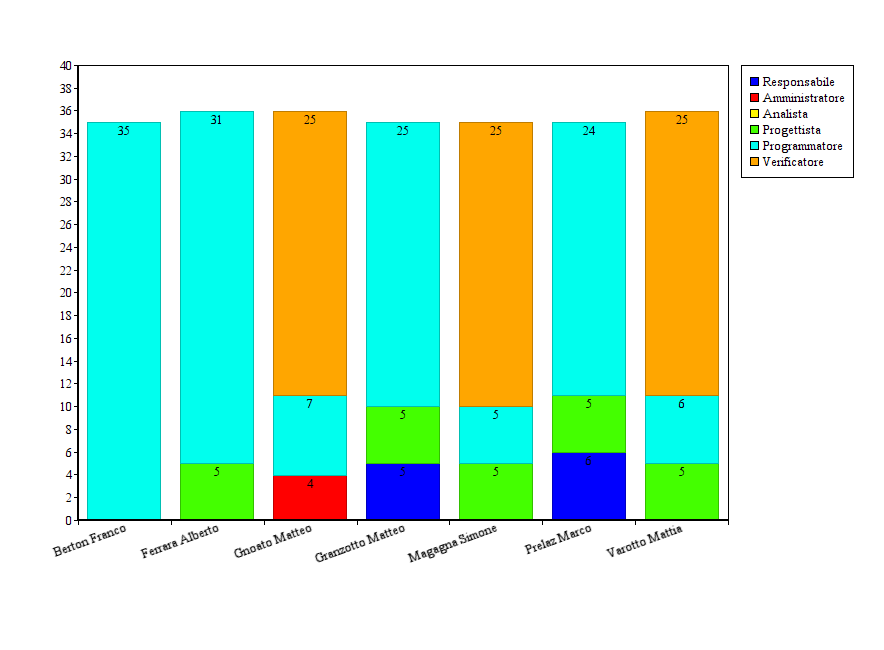
\includegraphics[scale=0.4]{immagini/Grafi/GrafoCod}
	\caption{Incidenza ore per ruolo, Codifica}
\end{figure}

\subsection{\VV}
Nel periodo di \VV{} ciascun componente del gruppo dovrà rivestire i seguenti ruoli:
\begin{table}[H]
	\begin{center}
		\begin{tabular}{|c|c|c|c|c|c|c|c|}
			\hline
			\textbf{Nominativo} & \multicolumn{6}{c|}{\textbf{Ore per ruolo}} & \textbf{Ore totali} \\
			& \textbf{Re} & \textbf{Am} & \textbf{An} & \textbf{Pj} & \textbf{Pr} & \textbf{Ve} & \\
			\hline
			\FB		&		&		&		&	6	&		&	11	&	17	\\
			\hline
			\AF		&		&		&		&	 6	&		&	11	& 	17	\\
			\hline
			\GN		&		&		&		&	8	&		&	9	&	17	\\
			\hline
			\GR	&		&	 	&		&		&	 	& 	18	&	18	\\
			\hline
			\SM 		&	9	&		&		&		&		& 	9	&	18	\\
			\hline
			\MP 		& 		&		&		&		&		&	18	&	17	\\
			\hline
			\MV 		&		&		&		&		&		&	17	& 	17	\\
			\hline
		\end{tabular}
	\end{center}
	\caption{Ore per componente, \VV}
\end{table}

\begin{figure}[H]
	\centering
	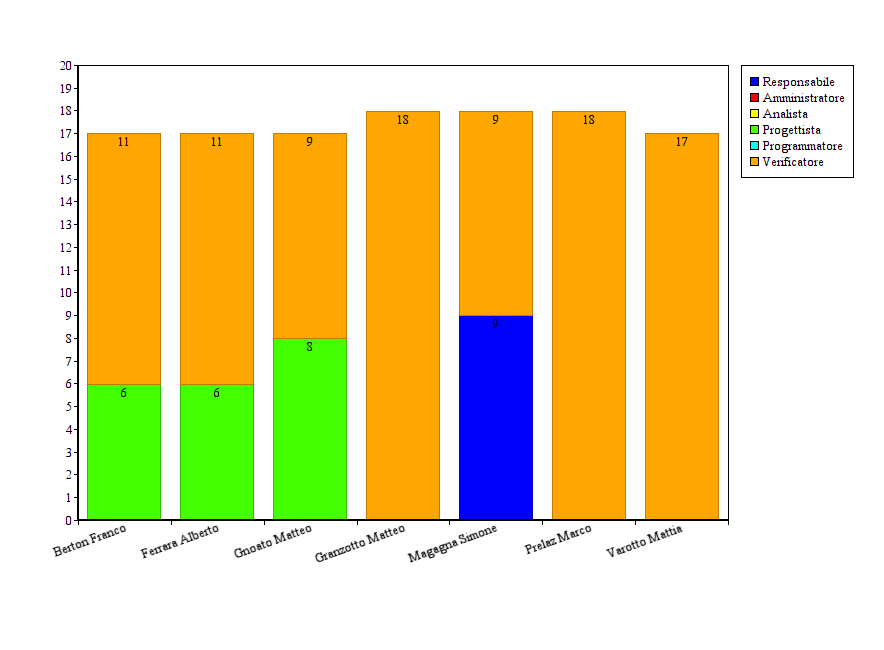
\includegraphics[scale=0.4]{immagini/Grafi/GrafoVV}
	\caption{Incidenza ore per ruolo, \VV}
\end{figure}

\subsection{Totali}
La tabella seguente illustra le ore totali che ogni componente dedicherà per il progetto, mettendo in evidenza anche quelle che verranno poi rendicontate.
\begin{table}[H]
	\begin{center}
		\begin{tabular}{|c|c|c|c|c|c|c|c|c|}
			\hline
			\multirow{2}{*}{\textbf{Nominativo}} & & \multicolumn{6}{c|}{\textbf{Ore per ruolo}} & \multirow{2}{*}{\textbf{Ore totali}} \\
			& & \textbf{Re} & \textbf{Am} & \textbf{An} & \textbf{Pj} & \textbf{Pr} & \textbf{Ve} & \\
			\hline
			\hline
			\multirow{2}{*}{\FB}		&	Rendicontate	&	3	&	0	&	0	&	33	&	35	& 34 	&	105	\\
			\cline{2-9}
			&	Totali			&	3	&	4	&	26	&	33	&	35	& 	34	&	135	\\
			\hline
			\hline
			\multirow{2}{*}{\AF}	&	Rendicontate	&	4	&	0	&	0	&	35	&	31	&  34	&	105	\\
			\cline{2-9}
			&	Totali			&	4	&	6	&	24	&	35	&	31	& 	34	&	135	\\
			\hline
			\hline
			\multirow{2}{*}{\GN}	&	Rendicontate	&	0	&	6	&	0	&	34	&	7	&	58	&	105	\\
			\cline{2-9}
			&	Totali			&	21	&	6	&	9	&	34	&	7	&	58	&	135	\\
			\hline
			\hline
			\multirow{2}{*}{\GR}	&	Rendicontate	&	5	&	4	&	0	&	39	&	25	&	32	&	105	\\
			\cline{2-9}
			&	Totali			&	27	&	4	&	8	&	39	&	25	&	32	&	135	\\
			\hline
			\hline
			\multirow{2}{*}{\SM}		&	Rendicontate	&	12	&	3	&	0	&	51	&	5	& 	34	&	105	\\
			\cline{2-9}
			&	Totali			&	12	&	7	&	5	&	51	&	5	& 	55	&	135	\\
			\hline
			\hline
			\multirow{2}{*}{\MP}	&	Rendicontate	&	6	&	4	&	0	&	39	&	24	& 	32	&	105	\\
			\cline{2-9}
			&	Totali			&	6	&	4	&	7	&	39	&	24	& 	55	&	135	\\
			\hline
			\hline
			\multirow{2}{*}{\MV}	&	Rendicontate	&	3	&	0	&	0	&	40	&	6	& 	56	&	105	\\
			\cline{2-9}
			&	Totali			&	3	&	4	&	5	&	40	&	6	& 	77	&	135	\\
			\hline
		\end{tabular}
	\end{center}
	\caption{Ore per componente per ruolo, rendicontate e totali}
\end{table}
